%% galaxies.tex

The current scientific consensus within the cosmological paradigm is that all
matter in the Universe was created roughly a Hubble time ($\Ho^{-1} =
13.7\;\Gyrs$) ago during a singularity known as the Big Bang.  Afterwards, a
rapidly expanding and cooling phase began, and all matter was almost uniform in
distribution.  Over the course of these several billion years, spontaneous
fluctuations on top of this uniform distribution grew, slightly denser regions
of matter became gravitationally bound to each other.  Eventually, they formed
primordial galaxies of hydrogen gas enveloped by a large dark matter halo.  In
these proto-galaxies, cold and over-dense molecular clouds gravitationally
collapsed to form the first stars.  These stars were rather massive and burnt
through their hydrogen fuel quickly.  Such stars generally end in violent
supernovae through which they reintroduce heavier elements\sidenote{commonly
termed \textit{metals} in astrophysics whose aggregates form \textit{dust}} back
into their gas environment, the \textit{interstellar medium} (ISM).  The
interplay of these components form a dynamical, self-regulatory, but chaotic
system and settle into a morphological state of the galaxy.  The study of these
dynamical processes and their correlations therefore can uncover crucial clues
to the formation history and structure of galaxies. 

The endeavour of measuring the dynamics of galaxies was and still is
complicated, even more so within the Milky Way.  Earth is revolving around our
Sun, and the Solar System is orbiting around the Galactic centre, which means
relative motions have to be carefully examined.  From some locations on Earth, a
dense strip of starlight is visible across the night sky which is indicative of
the Galaxy's disk structure.

\begin{figure}[h]
    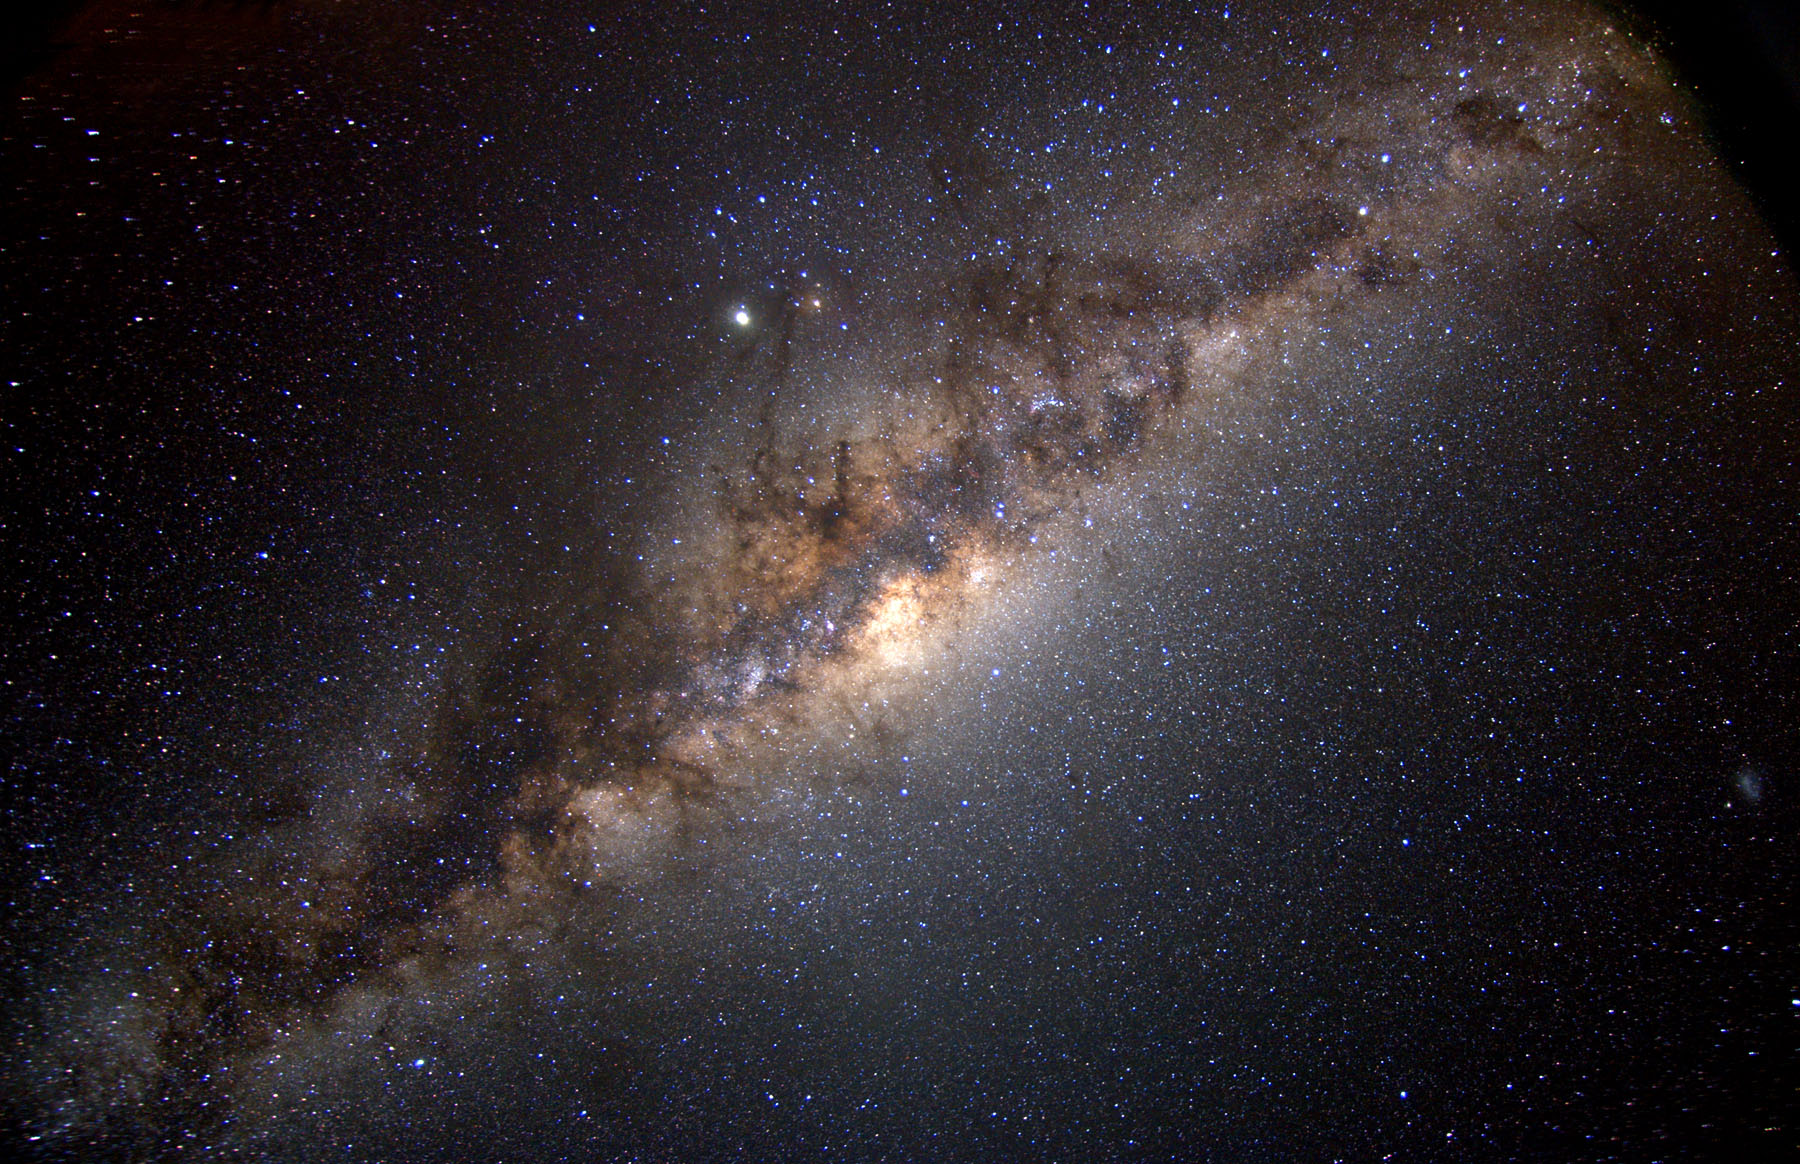
\includegraphics{apod080104}
    \caption[The Milky Way: APOD 2008 January
    4]{\href{https://apod.nasa.gov/apod/ap080104.html}{APOD 2008 January 4}: The
    Milky Way at 5000 meters.\\
    View on our own galaxy from within (recorded in the Chilean Andes).  The
    band of the dense collection of stars from the disk and the Galactic centre
    is partially covered by the typical extinction features due to dust
    clouds.  It indicates that the Milky Way possesses a stellar disk.\\
    \textit{Credit \& Copyright: Serge Brunier}}
    \figlbl{milkyway}
\end{figure}

From far away it is quite easy to recognise the typical morphology of other
galaxies through direct observations\sidenote{provided the telescope has enough
angular resolution}.  Measuring their rotational properties already becomes
increasingly difficult, but deducing the shape and rotation patterns of the
Milky Way from within is an undertaking of its own.

A seemingly random and dense distribution of stars as it appears in galaxies
should in principle collapse towards its potential well.  Despite the expansion
of the Universe, this would eventually lead to the collapse of entire galaxies
into their centres.  Like in many other astrophysical scenarios, pressure
gradients can take a stabilising role, balance gravity, and thereby prevent
complete collapse.  These balancing pressures depend on different physical
processes and generally define limiting scales.  For some galaxies, e.g.
ellipticals, the stars' random motions are the dominant drivers towards
stability, for spiral galaxies it is the rotation about their disk's centre.  In
contrast to orbiting systems such as the Sun and Earth, where most of the mass
is located near the guiding centre of the orbits, the Milky Way's mass
distribution is more complex and extended with different elements such as
various forms of hydrogen gas, dust, stars, and stellar remnants.  In general,
the study of galactic rotation through stars can yield insights not only into
the galaxy's morphology, but also into its formation history and mass
composition.  

Weighing galaxies is not an easy task either, partially because most of their
components are invisible, dark matter being the most elusive amongst them.
However, much like tree branches move in the wind, orbits of stars still feel
the gravitational pull from the mass inside them, independent of the nature of
the matter.  Stars in a more massive galaxy will move with higher orbital speeds
than in lower-mass galaxies; more formally, the mass $M$ inside the (circular)
orbit of radius $r$ is $M(<r) \propto V^{2}r$, where $V$ is the orbital speed of
the star.  Accordingly, by measuring the velocities of stars at a particular
distance from the centre, a mass estimate for the galaxy can be calculated,
which is a simple application of Newton's first law combined with Kepler's law.
It is equivalent to assuming the galaxy is in hydrostatic equilibrium formulated
by the virial theorem 
\begin{equation}
    \begin{aligned}
        &V^{2} = \frac{GM(<r)}{r}\\
        &2E = -U,
    \end{aligned}
\end{equation}
where $E$ and $U$ are the kinetic and potential energy respectively
\sidecite{BinneyTremaine08, Zwicky1933}.  When the individual orbits of stars
cannot be resolved in {e.g.} spiral galaxies, other 'tracers' can be used such
as atomic hydrogen gas measured through 21-cm line radiation in the radio
spectrum \sidecite{vandeHulst1951, Muller1951, vandeHulst1954}, or as
perturbations in the optical wavelengths.  For ellipticals, the velocity
dispersion $\sigma$ measured by the spread of spectral absorption lines is the
observable which analogously measures their mass as $M(<r) \propto \sigma^{2}r$
\sidecite{Schechter80, Davies83}.  The observables measured are, in most cases,
treated as dynamical equilibria, or temporal averages and therefore yield (by
implicitly assuming the ergodic theorem) 1-dimensional (1D) models such as the
rotation curve $V(r)$ \sidecite{Bosma17, Ablimit20, Cautun20}.  It characterises
the orbital velocity as a function of distance from the galactic centre. By
measuring how $V(r)$ behaves with increasing radius, we can draw conclusions
about the Milky Way's size, total mass, and the distribution thereof.  For
instance, a solid-body rotation $V \propto r$ would mean that the enclosed mass
ideally increases with $r^{2}$, Keplerian orbits go as $V \propto r^{-\half}$,
whereas $V \propto \text{const.}$ is a result of the enclosed mass increasing as
$r$.  This makes it a powerful tool to investigate the mass distribution of
galaxies.

However, on rare occasions, some galaxies can function as strong gravitational
lenses, and reveal even more details about their internal structure.  These rare
phenomena occur when a source aligns with a massive galaxy acting as a lens and
is multiply imaged or appears as an Einstein ring.  This depends on the
gravitational potential of the galaxy which in turn is related to its entire
mass and the distribution thereof.  As a consequence, the separation of the
images to the lens is determined by the mass inside (see the strong lensing case
of \eqref{lensing_types}), which is typically of the order of $1\,\arcsec$ for
galaxies at cosmological distances.  Moreover, lenses are rarely perfectly
aligned and circular in the real world, but have angular structure, which
produces distorted configurations of source images.  This is what allows us to
go beyond 1D models and infer a lens model in form of a 2D mass distribution
(more details on this are discussed in \secref{lensing}).  Hence, gravitational
lenses provide a unique opportunity to study distant galaxies and their
structure on scales which are difficult to infer with other methods.
Unfortunately, this type of analysis is limited to lensing systems which are
relatively rare, as previously mentioned.  To get an idea of just how rare such
lensing events are, we will next try to estimate the number of lensed sources
based on the Milky Way's rotation behaviour.

The Milky Way's rotation curve can be probed through its stars directly. To that
end, the relevant observables are the radial velocity $v_{z}$, the tangential
velocity $v_{t}$, distance from Earth $d$, and the longitude on the sky $l$.
Measurements of these quantities can be combined to the so-called \textit{Oort's
constants}
%
\begin{equation}\eqlbl{obs_oortsC}%
    \begin{aligned}%
        &A = \frac{v_{z}}{d\sin{2l}} \\
        &B = \frac{v_{t}}{d} - A\cos{2l}.
    \end{aligned}%
\end{equation}%
%
A caveat is the assumption that the stars, including the Sun, are on circular
orbits, which is only approximately true.  Moreover, it assumes the Milky Way
has a monotonically decreasing, symmetric potential.  Again, this is not
entirely true as spiral arms can introduce over-densities which manifest as
asymmetries and locally break monotonic behaviour in the potential.  Still,
within their limits the Oort's constants are very useful, because they can be
rewritten as
%
\begin{equation}\eqlbl{oortsC}
    \begin{aligned}%
        &A = -\frac{1}{2} \left[\frac{\derivd V}{\derivd r}
                                - \frac{V_{0}}{R_{0}}\right] \\
        &B = -\frac{1}{2}\left[\frac{V_{0}}{R_{0}}
                               + \frac{\derivd V}{\derivd r}\right].
    \end{aligned}%
\end{equation}
%
Recent measurements from the Gaia survey determined these constants with
$A=15.3\pm0.4\,\Oortsunitsalt$ and $B=-11.9\pm0.4\,\Oortsunitsalt$
\sidecite{Bovy17}.  These constants express the shear and vorticity of the disk
in the solar neighbourhood.  The shear essentially measures a deviation from
solid-body rotation, the vorticity how the angular momentum varies with small
changes in radius.  Adding both yields the velocity gradient $A+B =
-\frac{\derivd V}{\derivd r}$, which seems to be relatively flat with
$3.4\;\Oortsunitsalt$ as was expected from previous and alternative
investigations.  

From the velocity gradient the mass density for the Milky Way can be estimated
as follows
%
\begin{equation}\eqlbl{MWrho}
    \begin{aligned}
        \rho_{MW} &\quad\sim\quad \frac{(A+B)^2}{2\pi} \\
                  &\quad\sim\quad 10^{-33}\;\sec^{-2}
    \end{aligned}
\end{equation}
%
As a rough estimate, this is of the order of the total mass of the Milky Way
within its size volume $\sim M_{MW} / R_{MW}^3$, as long as the
assumptions of the Oort's constants are valid.  This is obviously not the case
outside the edge of the Galaxy.  However, the size of the Milky Way is not
clearly known.  The issue lies in the ambiguity regarding the definition of the
edge of the Galaxy.  In the literature the '$R_{200}$' is frequently used,
sometimes also called the 'virial' radius within which the mean density equals
200 times the cosmological critical density.  Another less back-of-the-envelope
definition is the 'splashback' radius, a caustic manifested in a drop in density
or radial velocity.  At roughly half the splashback radius an edge can be
defined where virialized material has completed at least two pericentric
passages.  For the Milky Way this radius is at about $R_{MW} \sim
290\;\mathrm{kpc}$ \sidecite{Deason20}, and seems to define an edge where our
assumptions should still hold. 

Generalizing and assuming that the Milky Way is an average galaxy in the
Universe, we can compare the mass density of the Milky Way to the cosmological
matter density
%
\begin{equation}
    \begin{aligned}
        \rho_{m} &=\quad 0.3\times\frac{3\Ho^{2}}{8\pi} \\
                 &\sim\quad 10^{-37}\;\sec^{-2},
    \end{aligned}
\end{equation}
%
which is roughly 30\% of the average energy-density in the Universe.  The ratio
of these two quantities should yield the number of Milky-Way-like galaxies
within the galaxy's volume. Within a cubic volume of $\sim (c/\Ho{})^{3}$ which
corresponds roughly to a tenth of the diameter of the observable Universe and
$10^4$ times farther than the edge of the Milky Way, this number is roughly
%
\begin{equation*}
    10^{12}\times\frac{\rho_m}{\rho_{MW}} \sim 10^{8}.
\end{equation*}
%
Typical strong-lensing galaxies cover roughly an area of $10^{-10}$ square
radians on the sky, which means that within a tenth of the observable Universe
1\% of sources are strongly lensed by galaxies.  Of course, this number is based
on the mass and dimensions of the Milky Way and with it the assumption our
Galaxy be average.  Since the Milky Way is actually more massive than the
average galaxy, the estimate constitutes a lower limit. 

It was further implicitly assumed all galaxies are distributed homogeneously and
isotropically within the considered volume.  These are structural consequences
of what is known as the \textit{cosmological principle}.  It states that on a
sufficiently large scale the properties of the Universe are the same for all
observers, which is equal to say that the same physical laws apply throughout.
Extensive testing of these fundamental postulates to the measurable level seem
to confirm\sidenote{although not conclusively; see \citeay{Migkas20} for a
report of possible deviations from isotropy.} a statistically homogeneous
distribution of galaxies on large scales.  On local scales however, the picture
is much more interesting.  The $\Lambda$CDM model predicts clustering along
filamentary structures within a web-like system of dark matter strings.  Once
formed, galaxies evolved together in larger galactic structures called groups,
clusters and superclusters.  Over time, gravity within these systems forces them
closer and closer, until they eventually collide in a series of mergers. The
outcome of these mergers depends on the mass of the galaxies in the collision.
Smaller 'dwarf' galaxies can be disrupted by larger ones and turned into streams
of stars which orbit the galactic core.  When large galaxies of similar size
come together, their spiral structure is generally lost, and the merged galaxies
become a giant elliptical galaxy.  Through these mergers, a hierarchical
spectrum of various galaxy types forms.

Ultimately, all galaxies within a group or cluster will eventually become
gravitationally bound to each other and merge into a giant elliptical galaxy.
Such almost or fully merged systems are known as 'fossil groups'. They are
always dominated by a single, very luminous and thus massive central galaxy,
around which other galaxies are at least two magnitudes less luminous and
therefore much smaller.  During their comparatively fast merging process, the
intra-group gas medium heats up.  Cooling times in these regions are much higher
than a Hubble time, and thus a large-scale X-ray halo around the original main
galaxy remains.  Fossil groups which have already fully merged, appear today as
massive, completely isolated elliptical galaxies with such group-like X-ray
halos.  As a final product of galaxy merging within a galaxy group, the mass
range of such fossil group galaxies starts at $\sim10^{13}\;\Msol$ and exceeds
the average mass of galaxies by orders of magnitude.  

In recent years, ever more elaborate large-scale hydrodynamical and N-body
simulations have been implemented, which displayed such hierarchical merging
schemes, and produced incredibly realistic galaxies.  Simulations generally use
the field of density fluctuations analogous to the ones observed in the CMB as
initial conditions and progress the entire system in time according to the
cosmological concordance model.  They demonstrate that galaxy formation is
driven by the growth of the underlying large-scale structure and the formation
of dark matter haloes.  Galaxies form through condensation of gas at the centres
of the potential wells of these dark haloes.  The galaxies' subsequent evolution
is usually governed by a plethora of sub-grid models which are adapted to
reproduce properties due to astrophysical effects below the resolution level
such as supernova winds and quasar feedback, in this context often called
\textit{AGN} (active galactic nucleus) feedback.  Based on theoretical
predictions from such simulations, physical properties of galaxies related to
baryons \sidenote{a collective term for all luminous matter in order to
differentiate it from dark matter and dark energy.} should be naturally in tight
correlation with the mass of the dark haloes by which they are hosted.  In
particular, the total mass in stars contained in galaxies reveals interesting
behaviour of how star formation is regulated within, when compared to the mass
of their dark matter halos.

\textit{Halo abundance matching} is a technique which allows such a comparison
and results in an empirical correlation between galaxy and halo properties
\sidecite{Moster12}.  Following an Occam’s razor approach, the technique
directly matches observed galaxy number densities for a given property (such as
luminosity) to theoretical halo number densities obtained through simulations.
The latest Planck survey \sidecite{Planck18b} measured a baryonic-to-total mass
ratio of $\Omega_{b}/\Omega_{m} \sim 0.14$ within the $\Lambda$CDM model.  If
light 'traces' mass this cosmological average should hold for galaxies of all
masses.  Abundance-matched galaxies however indicate that on small scales light
does no longer simply trace mass and predict the star formation of galaxies to
be suppressed at both the low and high ends of the mass spectrum, due to various
astrophysical effects such as tidal stripping\sidenote{depletion of a galaxy's
gas and stellar mass reservoir due to strong tidal forces from neighboring
galaxies}, Supernovae and AGNs.  Generally, having more concentrated baryonic
matter will increase the stellar-to-halo mass fraction while astrophysical
feedback processes which disperses baryonic matter decreases it.  Supernovae
have the tendency to impact galaxies with lower halo masses the strongest by
kinematically removing gas from star-forming regions, whereas AGNs are
especially effective in preventing the formation of stars in higher mass
galaxies through heating and dispersing of the star-forming gas.

In contrast to abundance matching and similar methods which usually rely purely
on theoretical predictions of the halo mass number density, lensing provides
once again an alternative to compare mass components of galaxies based on
observational estimates.  Since lenses can be used to probe the distribution of
every kind of matter in galaxies, especially within the , masses
inferred by lens models represent a lower limit on the total mass of a galaxy.  


% stellar kinematics and colours of the stellar population in the lensing galaxy


%%%%%%%%%%%%%%%%%%%%%%%%%%%%%%%%%%%%%%%%%%%%%%%%%%%%%%%%%%%%%%%%%%%%%%%%%%%%%%%%	
\par\noindent\rule{\textwidth}{0.8pt}




\begin{figure}[h]%
    \centering%
    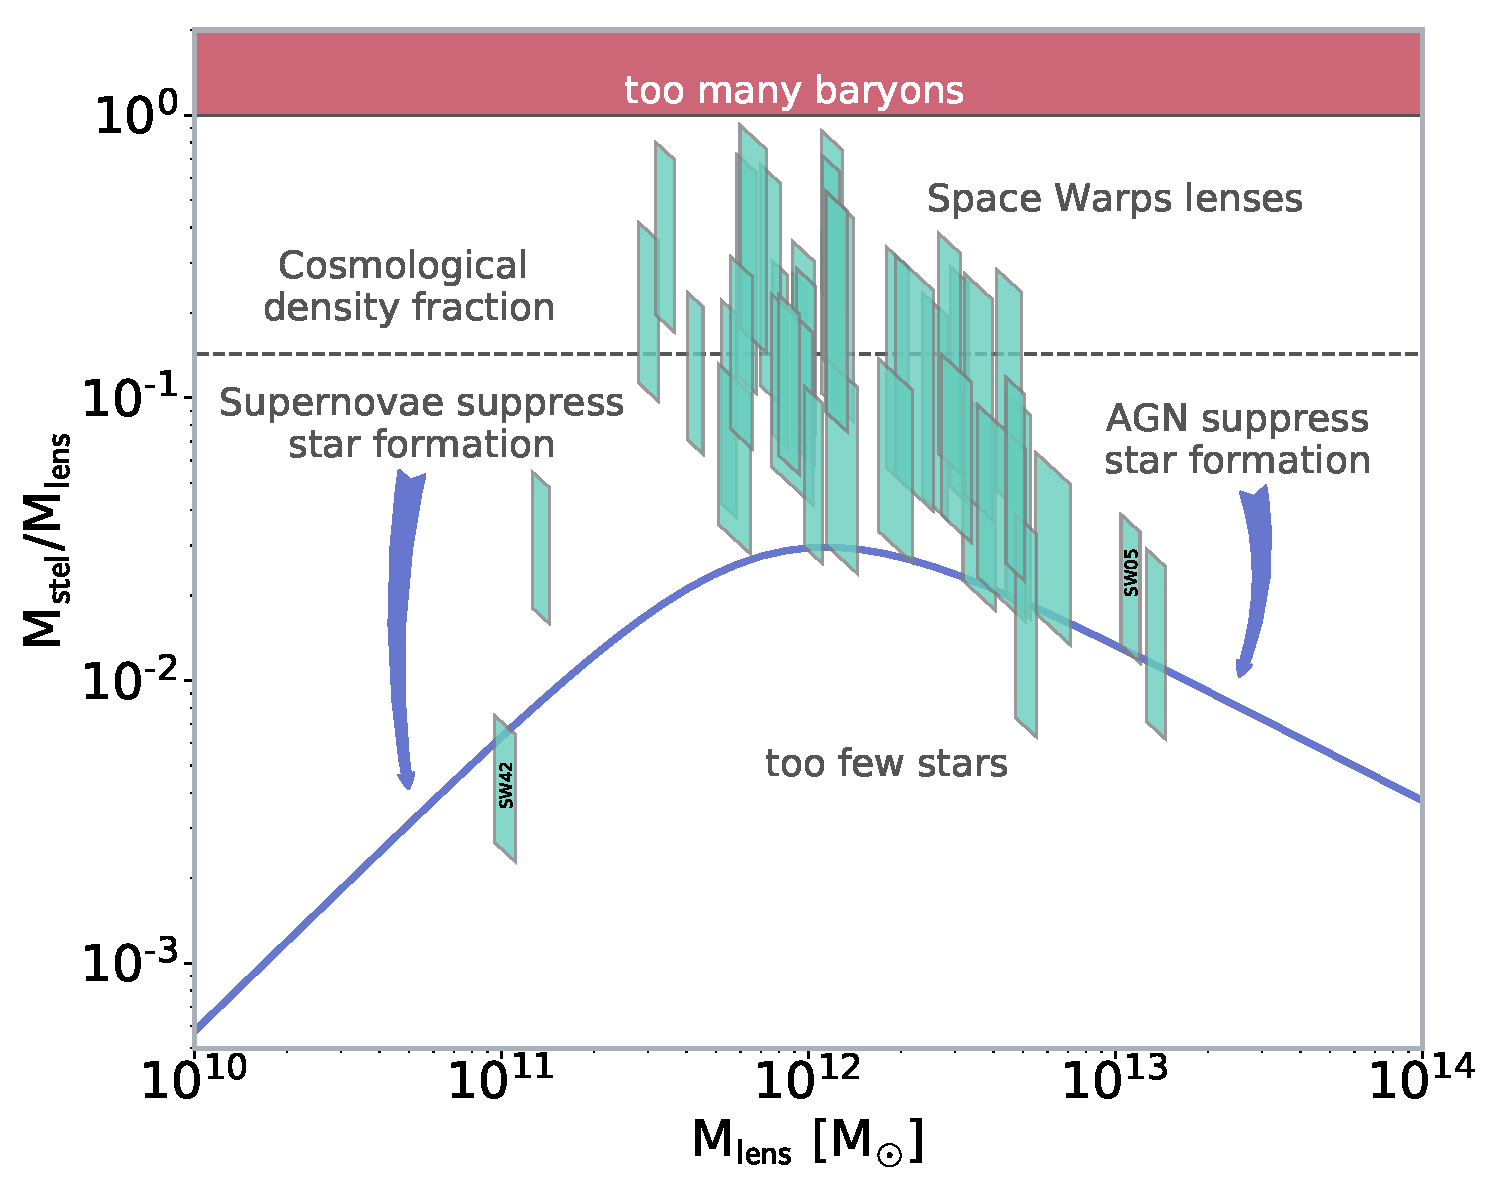
\includegraphics[width=0.99\textwidth]{moster}%
    \caption[Stellar-to-lens mass ratios of lensing galaxies]{Stellar-to-lens
        mass ratios of lensing galaxies (turquoise) from the
        Canada-France-Hawaii Telescope Legacy Survey (CFHTLS) in comparison with
        abundance-matched halo masses \cite[blue line; cf. Moster et
        al.][]{Moster12} and the cosmological density fraction
        $\Omega_{b}/\Omega_{m}$ (dashed line).  The lenses were discovered by
        the Space\,Warps citizen-science community and modelled by a smaller
        group of volunteers using the SpaghettiLens software stack by
        \citeay{SpL-stack}.  \citeay{Kueng18} presented their final results and
        estimated stellar-mass contents obtained through comparison with stellar
        populations.  The annotated lens models SW05 and SW42 have been refined
        by me (and collaborators) using Markov-chain Monte-Carlo simulations to
        marginalize over various sets of stellar population synthesis models,
        yielding much preciser stellar-mass and lens-mass estimates; for details
        see \chref{fossil}.  }%
    \figlbl{moster}%
\end{figure}%